

\section{Traditional Certification Frameworks Composition}
Modern certification frameworks rely upon several components defining how the process is executed and how the results should look. Below is a detailed list of the major pillars of certification frameworks with their fundamental functionalities as underlined by Anisetti et al. \cite{anisetti2017semi}\cite{anisetti2022multi}.

\subsection{Non-Functional Properties}
For the certification process of a system, it is important to establish some requirements that can be functional or non-functional preemptively, usually this is done during an initial risk assessment process. As stated by Chen et al. \cite{chen2013verification}: "broadly, functional requirements define what a system is supposed to do, and non-functional requirements define how a system is supposed to be", meaning that non-functional requirements focus on the system itself instead of what the system produces in output; once a requirement is proven to be satisfied by the system, it becomes a non-functional property of the same, and it can be expressed as follows: ⟨name, {(attribute, value), (attribute, value)}⟩. A property is composed of pairs "attribute-value" where the attributes are essential sub-properties that define the strength of the property.

In other words, non-functional properties describe the system's capabilities and are usually grouped under the categories defined by the CIA triad: i) Confidentiality, ii) Integrity and iii) Availability. The CIA triad is an organizational model designed to guide information storing policies; its three parts are cybersecurity's three most crucial components.

These properties are considered abstract because they represent generic security requirements and provide no information on how to achieve them. Instead, they are used to define concrete security properties. 

As defined by Anisetti et al. \cite{anisetti2013test}, a concrete security property is formally defined as follows:
A concrete security property, denoted \(p\), is a pair \( ( \hat{p}, A) \), where \(\hat{p}\) is an abstract property and \(A\) is a set of class attributes specifying the threats the service proves to counteract or the specific characteristics of the security function implemented by the service.

The NIST defined these components as follows \cite{pub2005minimum}:
\begin{description}
    \item[Confidentiality] Preserving authorized restrictions on information access and disclosure, including means for protecting personal privacy and proprietary information.
    \item[Integrity] Guarding against improper information modification or destruction, and includes ensuring information non-repudiation and authenticity.
    \item[Availability] Ensuring timely and reliable access to and use of information.

\end{description}

Confidentiality is a set of rules that limits access to information; ensuring confidentiality means the authorized entities can access the protected information and the unauthorized entities cannot. Confidentiality is accomplished through methods like data encryption and authentication procedures.

Integrity is the assurance that the information is trustworthy and accurate; it involves maintaining data consistency and accuracy over its entire lifecycle. For example, measures like file permissions and user access control ensure unauthorized entities cannot change data, while checksums and backups safeguard data from non-human threats like electromagnetic pulses or server crashes.

Availability guarantees reliable access to the information; it is best ensured by rigorously maintaining all hardware and staying up to date with all system upgrades; providing bandwidth, preventing bottlenecks and fast disaster recovery are also essential.

The NIST officially published several technical and non-technical capabilities that an IoT system’s manufacturer should consider; It should be noted that the following security requirements have been officially classified under one of the three parts of the CIA triad by the NIST.

Device identification, which is the capability to identify the IoT device for multiple purposes and in multiple ways to meet organizational requirements, is composed of the following requirements:

\begin{description}
    \item[Identifier Management Support] Ability for device identification. Elements that may be necessary:
        \begin{itemize}
            \item Ability to uniquely identify the IoT device logically.
            \item Ability to uniquely identify a remote IoT device.
            \item Ability for the device to support a unique device ID (e.g., to allow it to be linked to the person or process assigned to use the IoT device).
        \end{itemize}
    \item[Device Authentication Support] Ability to support local or interfaced device authentication. Elements that may be necessary:
        \begin{itemize}
            \item Ability for the IoT device to identify itself as an authorized entity to other devices.
            \item Ability to verify the identity of an IoT device.
        \end{itemize}
    \item[Physical Identifiers] Ability to add a unique physical identifier at an external or internal location on the device authorized entities can access.
\end{description}

On the other hand, the device configuration is defined as The capability to configure the IoT device through logical or physical interfaces to meet organizational requirements and includes the following requirements:
\begin{description}
    \item[Logical Access Privilege Configuration] Ability for only authorized entities to apply logical access privilege settings within the IoT device and configure logical access privilege as described in Logical Access to Interfaces.
    \item[Authentication and Authorization Configuration] Ability for only authorized entities to configure IoT device authentication policies and limitations as described in Logical Access to Interfaces.
    \item[Interface Configuration] Ability for only authorized entities to configure aspects related to the device’s interfaces as described in Logical Access to Interfaces.
    \item[Display Configuration] Ability to configure content to be displayed on a device.
    \item[Device Configuration Control] Ability to change configurations on the IoT device based on operational events as described in Device Security and Cybersecurity Event Awareness.
    \begin{itemize}
        \item Ability to change the device’s software configuration settings.
        \item Ability for authorized entities to restore the device to a secure configuration defined by an authorized entity.
        \item Configuration settings for use with the Device Configuration capability including, but not limited to:
        \begin{itemize}
            \item Ability for authorized entities to configure the cryptography use itself, such as choosing a key length.
            \item Ability to configure any remote update mechanisms to be either automatically or manually initiated for update downloads and installations.
            \item Ability to enable or disable notification when an update is available and specify who or what is to be notified.
        \end{itemize}
    \end{itemize}
\end{description}

Every IoT system revolves around data, and protecting it is the core focus of cybersecurity; the NIST defines data protection as the capability to protect IoT device data to meet organizational requirements. Therefore, it is important to satisfy as many of the following requirements as possible to achieve a high level of data protection.

\begin{description}
    \item[Cryptography Capabilities and Support] Ability for the IoT device to use cryptography for data protection. Elements that may be necessary:
        \begin{itemize}
            \item Ability to execute cryptographic mechanisms of appropriate strength and performance.
            \item Ability to obtain and validate certificates.
            \item Ability to verify digital signatures.
            \item Ability to run hashing algorithms.
            \item Ability to perform authenticated encryption algorithms.
            \item Ability to compute and compare hashes.
        \end{itemize}
    \item[Cryptographic Key Management] Ability to manage cryptographic keys securely:
        \begin{itemize}
            \item Ability to generate key pairs.
            \item Ability to store encryption keys securely.
            \item Ability to change keys securely.
        \end{itemize}
    \item[Secure Storage] Ability for the IoT device, or tools used through the IoT device interface, to enable secure device storage. Elements that may be necessary:
        \begin{itemize}
            \item Ability to support encryption of data at rest.
            \begin{itemize}
                \item Ability to cryptographically store passwords at rest, as well as device identity and other authentication data.
                \item Ability to support data encryption and signing to prevent data from being altered in device storage.
            \end{itemize}
            \item Ability to secure data in device storage
                \begin{itemize}
                    \item Ability to secure data stored locally on the device.
                    \item Ability to secure data stored in remote storage areas (e.g., cloud, server, etc.).
                    \item Ability to utilize separate storage partitions for system and user data.
                \end{itemize}
            \item Ability to “sanitize” or “purge” specific or all data in the device.
        \end{itemize}
        
    \item[Secure Transmission] Ability to secure data transmissions sent to and from the IoT device. Elements that may be necessary:
    \begin{itemize}
        \item Ability to configure the cryptographic algorithm to protect data in transit.
        \begin{itemize}
            \item Ability to support trusted data exchange with a specified minimum strength cryptography algorithm.
            \item Ability to support data encryption and signing to prevent data from being altered in transit.
        \end{itemize}
        \item Ability to utilize one or more capabilities to protect the data it transmits from unauthorized access and modification.
        \item Ability to use cryptographic means to validate the integrity of data transmitted.
    \end{itemize}
\end{description}

Another important aspect is the security of logical access to the system's interfaces, which is the ability to require authentication to or identify the IoT device and to establish authentication and identification configuration and display requirements.

\begin{description}
    \item[Authentication Support] Ability to support authentication methods.
    \begin{itemize}
        \item Ability for the IoT device to require authentication prior to connecting to the device.
        \item Ability for the IoT device to support and require appropriate authentication
        \begin{itemize}
            \item Ability for the IoT device to require authentication prior to connecting to the device.
            \item Ability for the IoT device to support a second, or more, authentication method(s) through an out of band path such as temporary passwords or other one-use logon credentials, third-party credential checks, biometrics, text messages, hard tokens and manufacturer proprietary methods
        \end{itemize}
        \item Ability for the IoT device to hide or mask authentication information during authentication process.
        \item Ability for the IoT device to support a second, or more, authentication method(s) through an out-of-band path such as: Temporary passwords or other one-use credentials; Third-party credential checks; Biometrics; Text messages; Hard Tokens; etc.
    \end{itemize}
    
    \item[Authentication Configuration] Ability to require, or not require, authentication to, and/or identification of, the IoT device, and to establish authentication and identification configuration and display requirements. Elements that may be necessary:
    \begin{itemize}
        \item Ability to set and change authentication configurations, policies and limitations settings for the IoT device
        \begin{itemize}
            \item Ability to set the time period for how long the device will remain locked after an established configurable limit of unsuccessful login attempts has been met.
            \item Ability to disable or lock access to the device after an established number of unsuccessful login attempts.
            \item Ability to display and/or report the previous date and time of the last successful login authentication.
            \item Ability to automatically disable accounts for the IoT device after an establish period of inactivity
            \item Ability to support automatic logout of inactive accounts after a configurable established time period.
            \item Ability to support automatic removal of temporary, emergency and other special use accounts after an established time period.
        \end{itemize}
        \item Ability to authenticate external users and systems
        \item Ability to revoke their access.
    \end{itemize}
    
    \item[System Use Notification Support] Ability to support system use notifications.
    \begin{itemize}
        \item Ability to display to IoT device users an organizationally-defined system use notification message or banner prior to successful IoT device authentication. (e.g., the message or banner would provide privacy and security notices consistent with applicable federal laws, Executive Orders, directives, policies, regulations, standards, and guidance).
        \item Ability to create an organizationally-defined system use notification message or banner to be displayed on the IoT device
        \begin{itemize}
            \item Ability to edit an existing IoT device display.
            \item Ability to establish the maximum size (in characters, bytes, etc.) of the available device display.
        \end{itemize}
        \item Ability to keep the notification message or banner on the device screen until the device user actively acknowledges and agrees to the usage conditions
    \end{itemize}
    
    \item[Authorization Support] Ability to restrict all unauthorized interactions.
    \begin{itemize}
        \item Ability to identify authorized users and processes.
        \item Ability to differentiate between authorized and unauthorized users (physical and remote).
    \end{itemize}
    
    \item[Authentication And Identity Management] Ability to establish access to the IoT device to perform organizationally-defined user actions without identification or authentication.
    
    
    \item[Role Support And Management] Ability to establish unique, privileged, organization-wide, and other types of IoT device user accounts. Elements that may be necessary:
    \begin{itemize}
        \item Ability to create unique IoT device user accounts.
        \item Ability to assign roles to IoT device user accounts.
        \item Ability to identify unique IoT device user accounts.
        \item Ability to support a hierarchy of logical access privileges for the IoT device based on roles (e.g., admin, emergency, user, local, temporary, etc.).
        \begin{itemize}
            \item Ability to establish user accounts to support role-based logical access privileges.
            \item Ability to administer user accounts to support role-based logical access privileges.
            \item Ability to use organizationally-defined roles to define each user account’s access and permitted device actions.
            \item Ability to support multiple levels of user/process account functionality and roles for the IoT device.
        \end{itemize}
        \item Ability to apply least privilege to user accounts (i.e., to ensure that the processes operate at privilege levels no higher than necessary to accomplish required functions).
        \begin{itemize}
            \item Ability to create additional processes, roles (e.g., admin, emergency, temporary, etc.) and accounts as necessary to achieve least privilege.
            \item Ability to apply least privilege settings within the device (i.e., to ensure that the processes operate at privilege levels no higher than necessary to accomplish required functions).
            \item Ability to limit access to privileged device settings that are used to establish and administer authorization requirements.
            \item Ability for authorized users to access privileged settings.
        \end{itemize}
        \item Ability to support organizationally-defined actions for the IoT device.
        \begin{itemize}
            \item Ability to create organizationally-defined accounts that support privileged roles with automated expiration conditions.
            \item Ability to establish organizationally-defined user actions for accessing the IoT device and/or device interface.
            \item Ability to enable automation and reporting of account management activities.
            \item Ability to assign access to IoT device audit controls to specific roles or organizationally-defined personnel.
            \item Ability to control access to IoT device audit data.
            \item Ability to identify the user, process or device requesting access to the audit/accountability information (i.e., to ensure only authorized users and/or devices have access).
            \item Ability to establish conditions for shared/group accounts on the IoT device.
            \item Ability to administer conditions for shared/group accounts on the IoT device.
            \item Ability to restrict the use of shared/group accounts on the IoT device according to organizationally-defined conditions.
        \end{itemize}
        \item Ability to implement dynamic access control approaches (e.g., service-oriented architectures) that rely on:
        \begin{itemize}
            \item run-time access control decisions facilitated by dynamic privilege management.
            \item organizationally-defined actions to access/use device.
        \end{itemize}
        \item Ability to allow information sharing capabilities based upon the type and/or role of user attempting to share the information.
        \item Ability to restrict access to IoT device software, hardware, and data based on user account roles, used with proper authentication of the identity of the user to determine type of authorization.
    \end{itemize}
    
    
    \item[Limitations on Device Usage] Ability to establish restrictions for how the device can be used. Elements that may be necessary:
    \begin{itemize}
        \item Ability to establish pre-defined restrictions for information searches within the device.
        \item Ability to establish limits on authorized concurrent device sessions for:
        \begin{itemize}
            \item User accounts
            \item Roles
            \item Groups
            \item Dates
            \item Times
            \item Locations
            \item Manufacturer established parameters
        \end{itemize}
    \end{itemize}
    
    
    \item[External Connections] Ability to support external connections. Elements that may be necessary:
    \begin{itemize}
        \item Ability to securely interact with authorized external, third-party systems.
        \item Ability to allow for the user/organization to establish the circumstances for when information sharing from the device and/or through the device interface will be allowed and prohibited.
        \item Ability to establish automated information sharing to approved identified parties/entities.
        \item Ability to identify when the external system meets the required security requirements for a connection.
        \item Ability to establish secure communications with internal systems when the device is operating on external networks.
    \end{itemize}
    
    \item[Interface Control] Ability to establish controls for the connections made to the IoT device. Elements that may be necessary:
    \begin{itemize}
        \item Ability to establish requirements for remote access to the IoT device and/or IoT device interface including:
        \begin{itemize}
            \item Usage restrictions
            \item Configuration requirements
            \item Connection requirements
            \item Manufacturer established requirement
        \end{itemize}
        \item Ability to restrict use of IoT device components (e.g., ports, functions, microphones, video).
        \item Ability to logically or physically disable any local and network interfaces that are not necessary for the core functionality of the device.
        \item Ability to restrict updating actions to authorized entities.
        \item Ability to restrict access to the cybersecurity state indicator to authorized entities.
        \item Ability to restrict use of IoT device services.
        \item Ability to enforce the established local and remote access requirements.
        \item Ability to prevent external access to the IoT device management interface.
        \item Ability to control the IoT device’s logical interface (e.g., locally or remotely).
        \item Ability to change IoT device logical interface(s).
        \item Ability to control device responses to device input.
        \item Ability to control output from the device.
        \item Ability to support wireless technologies needed by the organization (e.g., Microwave, Packet radio (UHF/VHF), Bluetooth, Manufacturer defined)
        \item Ability to support communications technologies (including but not limited to):
        \begin{itemize}
            \item IEEE 802.11
            \item Bluetooth
            \item Ethernet
            \item Manufacturer defined
        \end{itemize}
        \item Ability to establish and configure IoT device settings for wireless technologies including authentication protocols (e.g., EAP/TLS, PEAP).
    \end{itemize}
\end{description}
    
    Given the intrinsic dynamicity of IoT systems and devices, software updates are frequent, and support mechanisms may need additional security properties. These requirements refer to the ability to update IoT device software and support mechanisms for such updates.
    \begin{description}
        \item[Update Capabilities] Ability to update the IoT device software within the device and/or through the IoT device interface. Elements that may be necessary:
        \begin{itemize}
            \item Ability to update the software by authorized entities only using a secure and configurable mechanism.
            \item Ability to identify the current version of the organizational audit policies and procedures governing the software update.
            \item Ability to restrict software installations to only authorized individuals or processes.
            \item Ability to restrict software changes/uninstallations to only authorized individuals or processes.
            \item Ability to verify software updates come from valid sources using an effective method (e.g., digital signatures, checksums, certificate validation, etc).
        \end{itemize}
        
        \item[Update Application Support] Ability to update the device’s software through remote (e.g., network download) and/or local (e.g., removable media) means
        \begin{itemize}
            \item If software updates are delivered and applied automatically:
            \begin{itemize}
                \item Ability to verify and authenticate any update before installing it
                \item Ability to enable or disable updating
            \end{itemize}
        \end{itemize}
    \end{description}
    
    
    %% skipping cybersecurity awareness %%
    
    Last but not least important is the device's security, defined as the capability to secure the IoT device to meet organizational requirements.
    
    \begin{description}
        \item[Secure Execution] Ability to protect the execution of code on the device. Elements that may be necessary:
        \begin{itemize}
            \item Ability to enforce organizationally-defined execution policies.
            \begin{itemize}
                \item Ability to execute code in confined virtual environments.
                \item Ability to separate IoT device processes into separate execution domains.
            \end{itemize}
            \item Ability to separate the levels of IoT device user functionality.
            \item Ability to authorize various levels of IoT device functionality.
        \end{itemize}
        
        
        \item[Secure Communication] Ability to securely initiate and terminate communications with other devices. Elements that may be necessary:
        \begin{itemize}
            \item Ability to enforce traffic flow policies.
            \item Ability to utilize standardized protocols.
            \item Ability to establish network connections.
            \item Ability to terminate network connections (e.g., automatically based on organizationally-defined parameters).
            \item Ability to de-allocate TCP/IP address/port pairings.
            \item Ability to establish communications channels.
            \item Ability to secure the communications channels.
            \item Ability to interface with DNS/DNSSEC.
            \item Ability to store and process session identifiers.
            \item Ability to identify and track sessions with identifiers.
        \end{itemize}
        
        \item[Secure Resource Usage] Ability to securely utilize system resources and memory. Elements that may be necessary:
        \begin{itemize}
            \item Ability to support shared system resources.
            \begin{itemize}
                \item Ability to release resources back to the system.
                \item Ability to separate user and process resources use.
                \item Ability to no one will read this.
            \end{itemize}
            \item Ability to manage memory address space assigned to processes.
            \item Ability to enforce access to memory space through the kernel.
            \item Ability to prevent a process from accessing memory space of another process.
            \item Ability to enforce configured disk quotas.
            \item Ability to continue operation when associated networks are unavailable (e.g., a smart smoke detector must still go off when a fire occurs even if it is not attached to the associated network).
            \item Ability to provide sufficient resources to store and run the operating environment (e.g., operating systems, firmware, applications).
            \item Ability to utilize file compression technologies (e.g., to provide denial of service protection).
        \end{itemize}
        
        
        \item[Device Integrity] Ability to protect against unauthorized changes to hardware and software. Elements that may be necessary:
        \begin{itemize}
            \item Ability to perform security compliance checks on system components.
            \item Ability to detect unauthorized hardware and software components.
            \item Ability to take organizationally-defined actions when unauthorized hardware and software components are detected (e.g., disallow a flash drive to be connected even if a USB port is present).
            \item Ability to store the operating environment (e.g., firmware image, software, applications) in read-only media (e.g., Read Only Memory).
        \end{itemize}
        
        \item[Secure Device Operation] Ability to operate securely and safely. Elements that may be necessary:
        \begin{itemize}
            \item Ability to keep an accurate internal system time.
            \item Ability to define various operational states.
            \item Ability to support various modes of IoT device operation with more restrictive operational states.
            \begin{itemize}
                \item “travel mode” for transit.
                \item “safe mode” for operation when some or all network security is unavailable.
                \item Others as determined necessary based on the purpose and goals for the IoT device.
            \end{itemize}
            \item Ability to define differing failure types.
            \item Ability to fail in a secure state.
            \item Ability to disable operations and/or functionality in the event of security violations.
            \item Ability to restrict components/features of the IoT device (e.g., ports, functions, protocols, services, etc.) in accordance with organizationally-defined policies.
            \item Ability to sense the environment and securely (i.e., preserving confidentiality, integrity, and availability of the device and its data) interface with the environment, either directly or through the IoT system. Examples include:
            \begin{itemize}
                \item Emergency shutoff mechanism
                \item Emergency lighting mechanism
                \item Fire protection mechanism
                \item Temperature and humidity mechanism
                \item Water damage protection mechanism
                \item Manufacturer defined capability
            \end{itemize}
        \end{itemize}
        
        
    \end{description}
    
    
    Moreover, Nasiri et al. \cite{nasiri2019security} defined a series of security requirements that manufacturers should consider (and develop) when designing IoT systems. These requirements are a high-level summary of the above that could be useful while showcasing examples of systems’ design. Although the research refers to healthcare IoT systems, many properties are still relevant for any kind of IoT system.
    
    \begin{description}
        \item[Identification and authentication] Identification guarantees the identity of all the entities before permitting them to interact with the resources of the IoT system. Authentication is the process of confirming the identity of a person or device before using the system resources. Devices and application authentication can prove that the interacting system is not an adversary and that data shared in networks is legal.
        
        \item[authorization (access control)] After user identity verification, access rights or privileges to resources should be determined so that different users can only access the resources required based on their tasks.

        \item[privacy] Privacy means that secrets and personal data of users should not be disclosed without consent. Therefore, the IoT system should be in accordance with privacy policies allowing users to control their private data.

        \item[accountability] In a health IoT system, accountability should ensure that the organization or individuals are obliged to be answerable or responsible for their actions in case of theft or abnormal event.

        \item[non-repudiation] Non-repudiation ensures that someone cannot deny an action that has already been done. It enables the users to prove the occurrence or non-occurrence of an event.

        \item[auditing] Auditing is the ability of a system to track and monitor actions continuously. All user activities should be recorded in sequential order, such as system login time and data modification.
        
        \item[data freshness] Data freshness means that data should be recent, ensuring that no old messages are replayed.

        

    \end{description}
    

\subsection{Non-Functional Mechanisms}
For a non-functional property to be proven, a non-functional mechanism, in the form of \( ( name, \{ attribute, value \} )\), must be implemented to execute the certification process under specific configurations. Moreover, the property is what the process needs to verify, and the mechanism is the tool the system offers to test such property \cite{anisetti2017semi}; the verification is usually done through tests in the form of \\ \( (mechanism, (codde to execute, expected results))\). Finally, it is important to note that the mechanisms need to be described in the system's documentation; this allows the accredited laboratory to analyze and test them during the manual review phases.


\subsection{Target Of Certification}
The application context and the system perimeter define the Target of the Certification (ToC); it describes the mechanisms on which the non-functional properties that need to be certified rely. Moreover, the evaluation of the certification scheme must verify the target’s (security) features. For example, in the Common Criteria process, the ToC (actually named Target of Evaluation) is accurately described in the Security Target Document.

\subsection{Evidence}
Evidence collection is the main step to proving that a given non-functional property is valid for a given ToC; it is important to note that evidence can be gathered by testing the service actively or passively. 
The property is finally assigned to the system when enough evidence is collected for a given requirement through well-aimed tests. 


\subsection{Life Cycle}
\begin{figure}[hb]
    \centering
    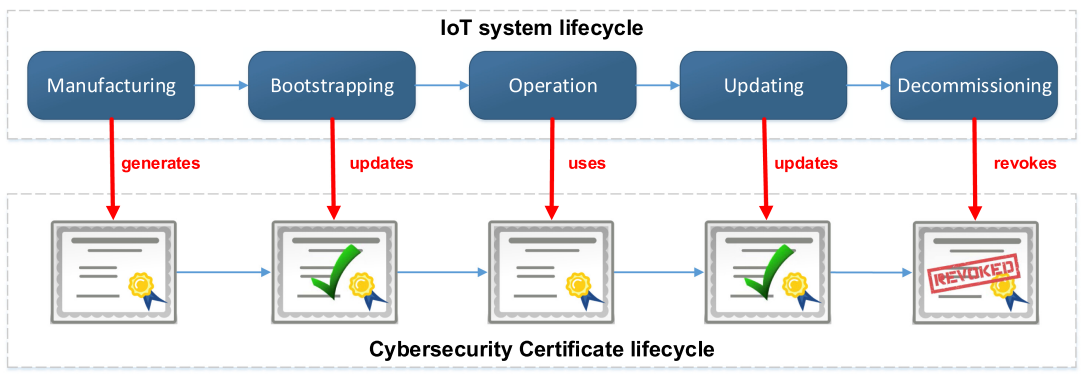
\includegraphics[scale=0.5]{images/lifeCycle.png}
    \caption{The cybersecurity certificate during the IoT device lifecycle.}
    \label{fig:lifecycle}
\end{figure}
As mentioned above, certificates are subject to invalidation, whether caused by a context change, a property change, or simply by the certificate's expiration; all certificates have a finite lifespan managed by the Certificate Authority (CA), which is usually also in charge of replacing it with a new one. However, the CA represents a bottleneck, and automation frameworks are needed when dealing with highly dynamic environments like Cloud and Edge. Therefore, the life cycle of a certificate is de facto a deterministic finite-state automaton whose state transitions are determined by specified conditions.

As mentioned above, certificates are subject to invalidation, whether caused by a context change, a property change, or simply by the certificate's expiration; all certificates have a finite lifespan managed by the Certificate Authority (CA), which is usually also in charge of replacing it with a new one. However, the CA represents a bottleneck, and automation frameworks are needed when dealing with highly dynamic environments like Cloud and Edge. Therefore, the life cycle of a certificate is de facto a deterministic finite-state automaton whose state transitions are determined by specified conditions.

As shown in figure \ref{fig:lifecycle}, the lifecycle of a certificate is tightly coupled with the lifecycle of the IoT system, which is usually divided into five phases: i) Manufacturing, ii) Bootstrapping, iii) Operation, iv) Updating and v) Decommissioning.

The manufacturing phase includes the production, programming and configuration of the system/device. This phase also includes the security certification process, which, if passed, assigns a brand new certificate to the system.

The bootstrapping phase includes the installation and configuration of the device for the specific domain in which it will operate. Moreover, context-specific information should be embedded in the cybersecurity label (this step is too often ignored). It is also important to note that the context plays a fundamental role in every IoT system; a given device could require different security levels based on the type of information it needs to handle, and this variation can happen multiple times in the lifespan of the device.

During the operation phase, the device/system provides its intended functionalities and should always be kept under a monitoring process. The monitoring is crucial to find new vulnerabilities and issues in the system. When a new vulnerability is found, and the manufacturer issues an update, rarely is a re-certification not issued due to the complexity of the analysis of the changes. Moreover, the security level and label are updated during a re-certification process.

The decommissioning phase represents the end of the lifecycle of the system and includes the certificate revocation. This phase is also crucial because the devices composing the system could have stored sensitive information, and this phase's sole purpose is to make such information inaccessible \cite{surveyIOT}.

Typically, a certification process for Cloud services consists of a collaborative effort between four entities: i) a service provider who develops the service that needs to be certified, ii) a cloud provider supporting the service's certification, iii) a CA responsible for the definition of the requirements and the methodology and iv) an accredited lab to carry out the system evaluation. The problem of such an approach resides in the fact that continuous context changes can rapidly invalidate the assigned certificates, and without proper context testing techniques, it is necessary to re-certificate the whole service every time. The framework that M. Anisetti et al. proposed addressed this issue by constantly verifying the possessed certifications against the context changes to prevent unnecessary revocations and re-certifications.


\subsection{Labels}
Labelling schemes exist to straightforwardly inform the user about the security certification that has been executed on a device; such schemes should contain the following main groups of information:

\begin{itemize}
    \item Domain that was considered while performing the certification activity; the certification should be revoked the moment the device leaves it

    \item Level of assurance; states the security tests performed to certify the device. Usually, the level of assurance is associated with the protection profile of the specific domain

    \item  Information about the achievement of the certification, such as the responsible entity, the process and the validity period

\end{itemize}

Even though the importance of labels is mostly tied to commercial purposes \cite{baldini2016security}, perhaps, they could also be read by the Certification Authorities to have a quicker overview of the system's mechanisms and capabilities. In state-of-the-art schemes, labels are ignored or poorly used, but they might play a fundamental role in future schemes.



